\documentclass[a4paper]{article}     
\usepackage{amsfonts}
\usepackage{amsmath}
\usepackage{amssymb}
\usepackage{graphicx}
\usepackage{cancel}

\newcommand{\asa}{\Leftrightarrow} %als slechts als
\newcommand{\adR}{\Rightarrow} %als dan Rechts
\newcommand{\adL}{\Leftarrow}
\newcommand{\Lh}{\left(} %Links haakje
\newcommand{\Rh}{\right)}
\newcommand{\Lv}{\left[} %Links vierkanthaakje
\newcommand{\Rv}{\right]}
\newcommand{\La}{\left\{} %Links acolade
\newcommand{\Ra}{\right\}}
\newcommand{\Ras}{\right.} %Rechts acolade stelsel (omdat om stelsels te maken heb je een punt nodig
\newcommand{\pnR}{\rightarrow} %pijl naar Rechts
\newcommand{\limiet}{\lim\limits_}
\newcommand{\schrap}{\cancel}
\newcommand{\schrapb}{\bcancel} %backslash
\newcommand{\schrapk}{\xcancel} %kruis
\newcommand{\vervang}{\cancelto}
\newcommand{\stijg}{\nearrow} %stelt stijgende pijl voor
\newcommand{\daal}{\searrow} %stelt dalende pijl voor

\begin{document}

\noindent \large Auteur: Yoren Collier \\
\noindent \large Studierichting: Informatica\\
\noindent \large Oefeningenreeks 3G nr. 9.3\\

\medskip

\normalsize

$f(x) = \dfrac{6x -3}{2x+5}$\\

1. dom, Im, periode, snijpunten assen\\

$\operatorname{dom} f = \mathbb{R} \setminus \La \dfrac{-5}{2} \Ra , \operatorname{Im} f = \mathbb{R}, \operatorname{per.} f = / $\\

$t(x) = 0 \asa 6x = 3 \asa x = \dfrac{1}{2}$ en $n(x) = 0 \asa 2x = -5 \asa x = \dfrac{-5}{2}$ met $t(x), n(x)$ respectievelijk de teller en noemer van de functie.\\

Snijpunt(en) $X$-as: $\Lh \dfrac{1}{2}, 0 \Rh$ , Snijpunt $Y$-as: $\Lh 0, \dfrac{-3}{5} \Rh$\\

Asymptoten:\\

VA: $\limiet{x \pnR \tfrac{-5}{2}} f(x) = \dfrac{\vervang{3}{6} \cdot \dfrac{-5}{\schrap{2}} -3}{\schrap{2} \cdot \dfrac{\schrapb{-5}}{\schrap{2}} + \schrapb{5}} = \dfrac{-18}{0}$\\

$\limiet{x \pnR \tfrac{-5}{2}-} f(x) = \dfrac{-18}{0^-} = +\infty$\\

$\limiet{x \pnR \tfrac{-5}{2}+} f(x) = \dfrac{-18}{0^+} = -\infty$\\

Ha: $\limiet{x \pnR \pm\infty} f(x) = \limiet{x \pnR \pm\infty} \dfrac{6\schrap{x}}{2\schrap{x}} = 3$\\

$f(x) -3 = \dfrac{6x -3}{2x+5} -3 = \dfrac{\schrap{6x} -3 -\schrap{6x} -15}{2x+5} = \dfrac{-18}{2x +5}$\\

\begin{tabular}{c|ccc}
        $x$&       &  $\dfrac{-5}{2}$  &     \\ \hline
     $f(x)$&  $-$  &  $|$              &  $+$
\end{tabular}

SA: 2 HA dus geen SA mogelijk.\\

Afgeleiden:\\

$\dfrac{df}{dx}(x) = \dfrac{\Lh 2x +5 \Rh \cdot 6 - \Lh 6x -3 \Rh \cdot 2}{\Lh 2x +5 \Rh ^2} = \dfrac{\schrap{12x} +30 - \schrap{12x} +6}{\Lh 2x +5 \Rh ^2} = \dfrac{36}{\Lh 2x +5 \Rh ^2}$\\

$\dfrac{d^2f}{dx^2}(x) = \dfrac{36 \cdot \Lh -2 \Rh}{\Lh 2x +5 \Rh ^3} \cdot 2 = \dfrac{-144}{\Lh 2x +5 \Rh ^3}$\\

\begin{tabular}{c|cc|c|c|c|cc}
     $x$&  $-\infty$  &            &  $\dfrac{-5}{2}$  &            &  $\dfrac{1}{2}$  &            &  $+\infty$\\ \hline
  $t(x)$&  $-$        &  $-$       &  $-$              &  $-$       &  $0$             &  $+$       &  $+$\\ \hline
  $n(x)$&  $-$        &  $-$       &  $0$              &  $+$       &  $+$             &  $+$       &  $+$\\ \hline
 $f'(x)$&  $+$        &  $+$       &  $|^{(2)}$        &  $+$       &  $+$             &  $+$       &  $+$\\ \hline
$f''(x)$&  $+$        &  $+$       &  $|^{(3)}$        &  $-$       &  $-$             &  $-$       &  $-$\\ \hline
  $f(x)$&  $3$        &  $+$       &  $|$              &  $-$       &  $0$             &  $+$       &  $3$\\
        &             &  $\stijg$  &                   &  $\stijg$  &                  &  $\stijg$  &  \\
        &             &  $\smile$  &                   &  $\frown$  &                  &  $\frown$  &  \\
\end{tabular}

Met $t(x)$ en $n(x)$ respectievelijk de teller en noemer van de oorspronkelijke functie. Ook is de grafiek boven de HA in $-\infty$ en onder de HA in $+\infty$ zoals af te leiden uit de eerdere tabel waar dit bestudeerd werd.\\

\begin{figure}[h]
\centering
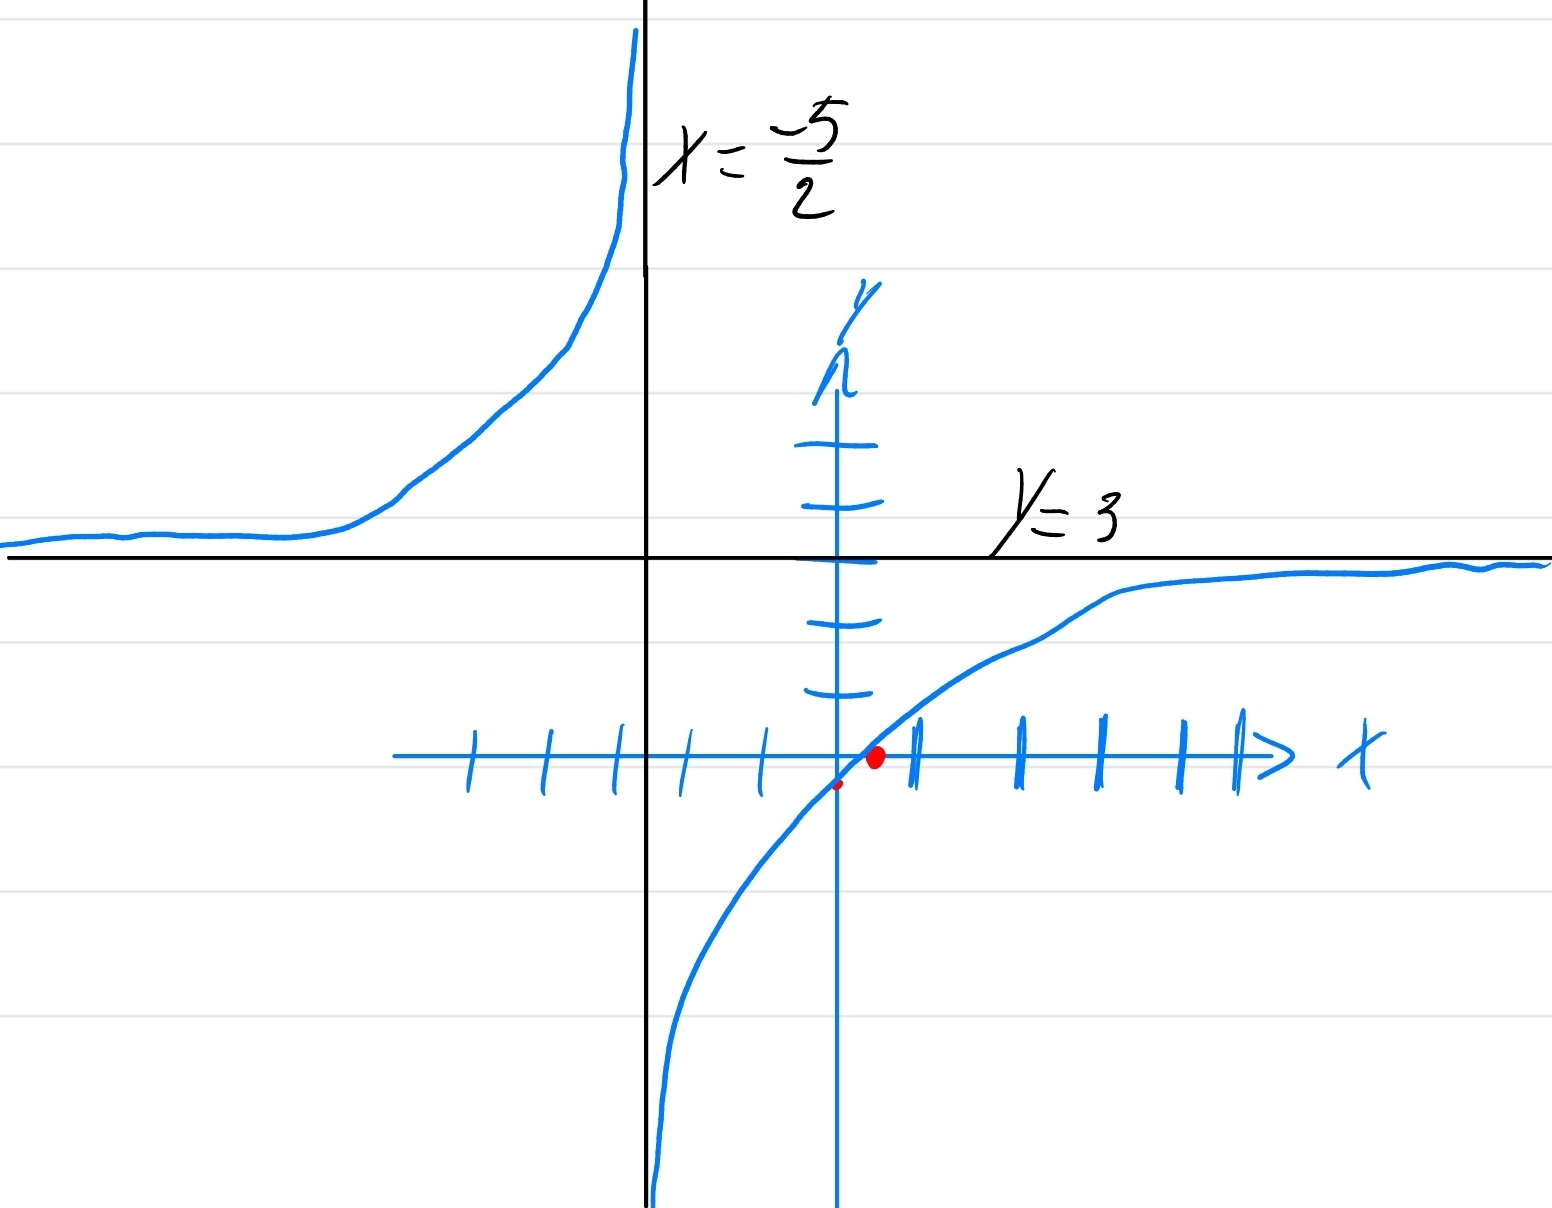
\includegraphics[width=10cm]{./3G-9.3-yoren.collier.INF.jpg}
\end{figure}

\begin{thebibliography}{999}
%\bibitem{a} Referentie
\end{thebibliography}
\end{document} 